% First draft (iteration 1). Generic two-column layout; swap in the venue template before submission.
\documentclass[10pt,twocolumn]{article}
\usepackage[margin=0.75in]{geometry}
\usepackage{graphicx}
\usepackage{booktabs}
\usepackage{amsmath}
\usepackage{hyperref}
\usepackage[numbers,sort&compress]{natbib}
\usepackage[font=small]{caption}

\title{Stock Arm, Printed Gripper: Validating Handheld Demonstrations\\
Against the Deployment Arm Before Training}
\author{Author names \quad Affiliation \quad \texttt{email}}
\date{}

\begin{document}
\maketitle

\begin{abstract}
Handheld UMI-style grippers make demonstrations cheap, but nothing in the
collection loop checks whether the robot that will run the policy can execute
them. We build the whole stack from parts that come with a commodity research
arm, the I2RT YAM (its MJCF model, its RealSense D405 wrist camera and an
open-source teleoperation IK), plus a 3D-printed handheld body carrying the same
D405 and a T265 tracker. Before training, every demonstration is replayed
through the arm's own deployment IK and follower in simulation and gated at
10\,mm / 5\textdegree. On a 10-episode session (6{,}024 frames) the stock
decoupled IK rejects 457 frames; a full-pose QP solver rejects 284, and its
accepted frames are 5$\times$ more accurate (p99 0.84\,mm vs.\ 4.63\,mm). We then
distil converged multi-start IK into a 9-input MLP that predicts reachability in
5\,\textmu s per pose, agrees with full IK on 99.8\% of real demonstration frames
and, by gradient ascent through the network, finds one rigid placement of the
demonstrations that makes every frame reachable (279\,$\to$\,0 unreachable,
verified by full IK). An ACT+CLIP policy trained on the collected data
picks and places a block on the arm. We report the latency budget of that
deployment and what remains unvalidated.
\end{abstract}

\section{Introduction}
UMI~\citep{chi2024umi} showed that a handheld gripper with a wrist camera can
replace teleoperation for collecting policy data, and FastUMI~\citep{zhaxizhuoma2024fastumi}
replaced SLAM with an off-the-shelf T265 tracker. Both leave one question to
deployment time: \emph{can the target arm actually follow the recorded hand
motion?} A human hand has no joint limits at the arm's wrist and no
non-intersecting wrist axes. When the arm cannot reach a training target, the
policy learns an action it will never execute, and the mismatch only shows up
on the robot.

We take the opposite route to building custom hardware: we use what ships with
a widely available low-cost arm and add only a printed handheld body. Because the
handheld and the robot share the same wrist camera model and the same kinematic
model, the arm's own software can audit the data. Our contributions:
\begin{itemize}
\setlength\itemsep{0pt}
\item An open handheld rig assembled from the YAM ecosystem (D405 wrist camera,
the arm's MJCF and IK) plus 3D prints and a T265, producing LeRobot~v3
datasets of relative end-effector trajectories.
\item \textbf{Deployment-in-the-loop validation}: each demonstration is replayed
through the deployment IK and 200\,Hz follower on a virtual arm; frames that
cannot be tracked are rejected before training.
\item \textbf{A learned workspace}: an MLP trained on 300k converged-IK labels
that answers reachability, expected error and an IK seed in one forward pass,
and a differentiable placement fit built on it.
\item An end-to-end deployment of ACT+CLIP on the arm with a measured latency
and tracking budget.
\end{itemize}

\begin{figure}[t]
\centering
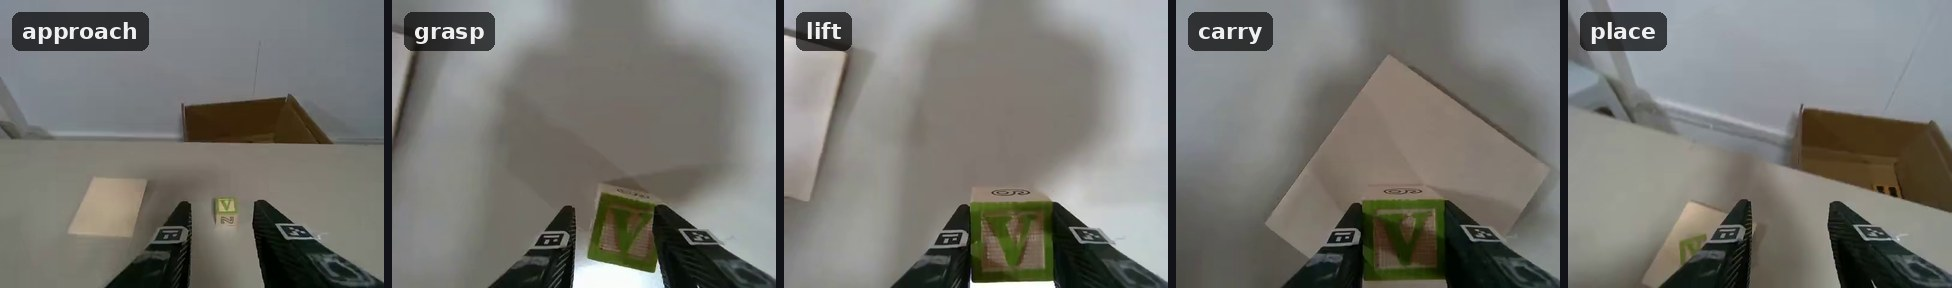
\includegraphics[width=\linewidth]{figures/training-demo-strip.jpg}\\[2pt]
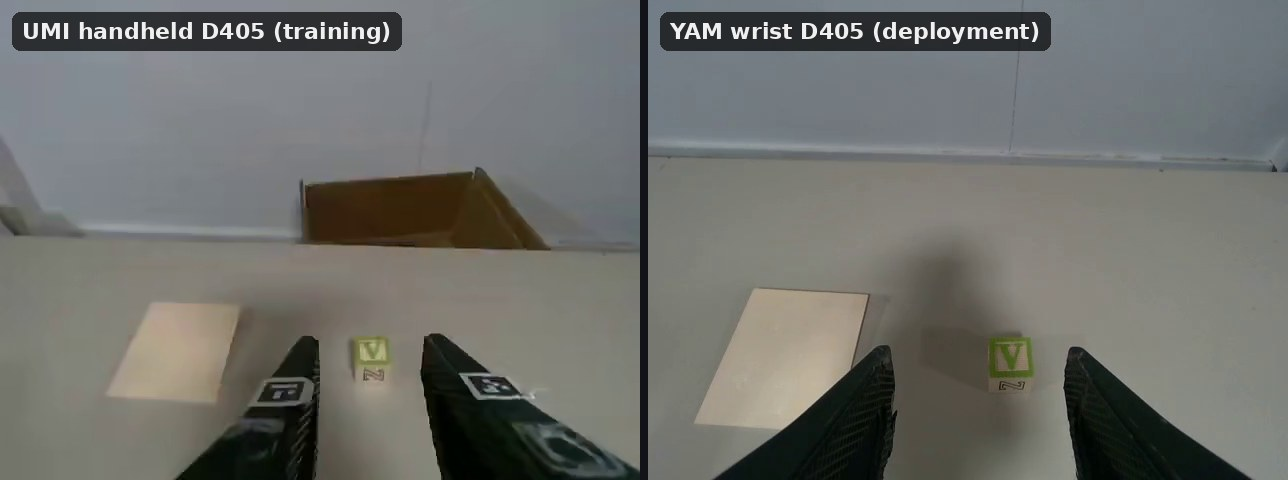
\includegraphics[width=\linewidth]{figures/umi-vs-yam-view.jpg}
\caption{Top: a handheld demonstration (approach, grasp, lift, carry, place).
Bottom: the handheld D405 view next to the YAM wrist D405 view at rollout start.}
\label{fig:rig}
\end{figure}

\section{System}
\textbf{Handheld.} A printed body holds a D405 (640$\times$480 at 30\,fps) and a
T265 (200\,Hz 6-DoF pose). Jaw width comes from two 10\,mm ArUco markers on the
fingers, read from the same image, so width and image are synchronized by
construction. D405 and T265 timestamps share the SDK global clock. Episodes are
stored as LeRobot~v3 with raw pose, IMU and depth.

\textbf{Arm.} The right arm of a bimanual YAM rig with its stock gripper and
wrist D405 is driven through Karma, an open teleoperation stack whose decoupled
IK solves position with joints 1--3 and orientation with joints 4--6, one
damped-least-squares step per 200\,Hz tick.

\textbf{Policy.} ACT~\citep{zhao2023act} with a fine-tuned CLIP~\citep{radford2021clip}
ViT-B/16 backbone predicts 50-step chunks of poses relative to the current pose,
$T_\text{now}^{-1}T_{k}$, plus absolute jaw width, from the wrist image and an
11-D state.

\section{Validating demonstrations on the deployment arm}
Each demonstration is mapped into the arm base frame with a gravity-aligned
anchor and streamed at 30\,Hz into the same follower and IK used on the robot.
A frame is rejected when the follower's tool pose misses the target by more than
10\,mm or 5\textdegree{}, or when the implied joint speed exceeds 3\,rad/s.
Table~\ref{tab:filter} shows a 10-episode block-placing session.

The stock decoupled IK is designed for teleoperation, where the operator closes
the residual: the YAM wrist axes do not intersect, so rotating the wrist leaves
up to $\sim$34\,mm of position error at the workspace edge. We replace it with a
full 6-DoF QP step (mink~\citep{zakka2024mink}, DAQP~\citep{arnstrom2022daqp}),
keeping the same per-tick joint caps as velocity limits, rotation weighted 0.1
(1\,rad $\approx$ 10\,cm) and a weak posture task (0.003) that keeps joints out of
limit corners. Without the posture task, joint 4 pinned at its limit (1{,}418
rejects); at 0.1 it overrode tracking (5{,}991). The solver runs in 0.1\,ms per
step and is a drop-in replacement.

\begin{table}[t]
\centering\small
\caption{Deployment-IK gate on session 20261008 (10 episodes, 6{,}024 frames;
3{,}339 frames have valid pose and width before IK). Errors are on frames both
solvers accept.}
\label{tab:filter}
\begin{tabular}{lccc}
\toprule
 & Decoupled & Full-pose QP & QP + placement \\
\midrule
IK rejects & 457 & 284 & \textbf{0} \\
Valid frames & 3{,}144 & 3{,}264 & \textbf{3{,}339} \\
Training chunks & 120 & 120 & 120 \\
Pos.\ err.\ p99 / max (mm) & 4.63 / 9.8 & \textbf{0.84 / 2.3} & -- \\
Rot.\ err.\ p99 / max (\textdegree) & 0.0 / 1.81 & 1.25 / 2.98 & -- \\
\bottomrule
\end{tabular}
\end{table}

The 284 remaining rejects, all in two episodes, are not a solver problem.
Converged multi-start IK cannot reach them either. Their positions are well
inside reach (0.53--0.59\,m from the shoulder, maximum 0.81\,m) and no joint
limit is active; the gripper approaches too close to vertical (median
22\textdegree{} from straight down, vs.\ 65\textdegree{} for accepted frames).
Moving those demonstrations 3/5/8\,cm toward the arm makes 39/50/57 of 57
sampled frames reachable; raising them makes none reachable. The data are
fine; their \emph{placement} relative to the arm is not. Training chunks do not
change (Table~\ref{tab:filter}) because marker dropouts, which affect 29\% of
frames, break contiguous windows first.

\section{A learned workspace}
Placement search, per-chunk checks at deployment and live feedback during
collection all need thousands of reachability queries per second, while
converged IK costs $\sim$10\,ms per pose. We distil it.

\textbf{Labels.} We sample 300k tool poses: 25\% forward kinematics of uniform
joint samples, 35\% those poses perturbed by $\mathcal{N}(0,5\,\text{cm})$ and
$\mathcal{N}(0,20^\circ)$ to populate the boundary, and 40\% uniform positions with
random orientations around the arm. A pose is \emph{reachable} if any joint
configuration within limits puts the tool within 10\,mm / 5\textdegree. The
reference solver needed three fixes to be trustworthy: (i) seeds from the 8
nearest poses in a 200k-entry forward-kinematics table before random restarts,
since random seeds missed a folded-elbow branch at joint 4's stop;
(ii) step-capped (0.15\,rad), damped iterations keeping the best iterate, since
full Newton steps left a 2\,mm solution for one 15\,cm away; and (iii) re-polishing
failures at several rotation weights, since a weighted optimum can lie outside
the tolerance box while another trade-off lies inside. After these fixes, 99.99\%
of forward-kinematics poses are labelled reachable and the reference never
loses to the deployment filter on real frames. Labelling takes 27\,min on 15 CPU
cores.

\textbf{Model.} Input is position plus the continuous 6-D rotation
representation~\citep{zhou2019continuity}. A 4$\times$256 SiLU trunk feeds three
heads: a reachability logit (BCE), $\log(1+\text{error})$ for position and
rotation (smooth-L1), and a joint seed (smooth-L1, reachable samples only).
Training takes 90\,s on CPU.

\begin{table}[t]
\centering\small
\caption{Learned workspace vs.\ converged IK.}
\label{tab:mlp}
\begin{tabular}{lcc}
\toprule
 & Held-out random & Real demo frames \\
\midrule
Poses & 30{,}000 & 6{,}024 \\
Accuracy & 98.5\% & \textbf{99.8\%} \\
AUC & 0.999 & 0.99997 \\
Missed unreachable & 0.85\% & 2 frames \\
False alarms & 0.70\% & 8 frames \\
Time per pose & \multicolumn{2}{c}{5.2\,\textmu s (MLP) vs.\ 9.9\,ms (IK), $\sim$1{,}900$\times$} \\
\bottomrule
\end{tabular}
\end{table}

\textbf{Uses.} (1) \emph{Placement fit}: a rigid shift $(\Delta x,\Delta y,\Delta z,\Delta\psi)$
of all demonstrations is optimized by Adam on the mean log-probability of
reachability, with a small cost per 10\,cm moved, from seven starts. In 4.5\,s it
finds $(-4.7, +0.3, -3.2)$\,cm and $-25.9^\circ$ yaw; full IK confirms 279\,$\to$\,0
unreachable frames, and the deployment filter then accepts every frame
(Table~\ref{tab:filter}). (2) \emph{Warm start}: seeding IK from the network's
joint head cuts the median iterations to converge from 5 to 1 on 400 demo frames.
(3) \emph{Review}: the replay viewer marks predicted-unreachable targets and
offers the placement fit with one click.

\section{Deployment}
The ACT+CLIP policy trained on 45 demonstrations (one held out) reaches a mean
position error of 36.7\,mm against the recorded chunk (73.6\,mm at the 1.67\,s
chunk end), 6.3\textdegree{} rotation and 1.5\,mm width on the held-out episode.
On the arm it reaches the block, closes to about 33\,mm and carries it over the
board. Figure~\ref{fig:latency} breaks down where error enters: inference takes
151--171\,ms, the first action leaves 254--290\,ms after the image, IK misses are
0.1\,mm, and the motors track commands with a 6.6--12.1\,mm median gap and
80--225\,ms joint lag; small commands on joints 3, 5 and 6 move in deadband steps.
Image-to-arm-in-place is $\sim$0.4\,s, i.e.\ 2--3\,cm at demonstration speeds.
Demonstration tempo is not the bottleneck: the median hand speed implies
0.3\,rad/s at the joints and only 8 of 6{,}014 frames exceed 3\,rad/s.

\begin{figure}[t]
\centering
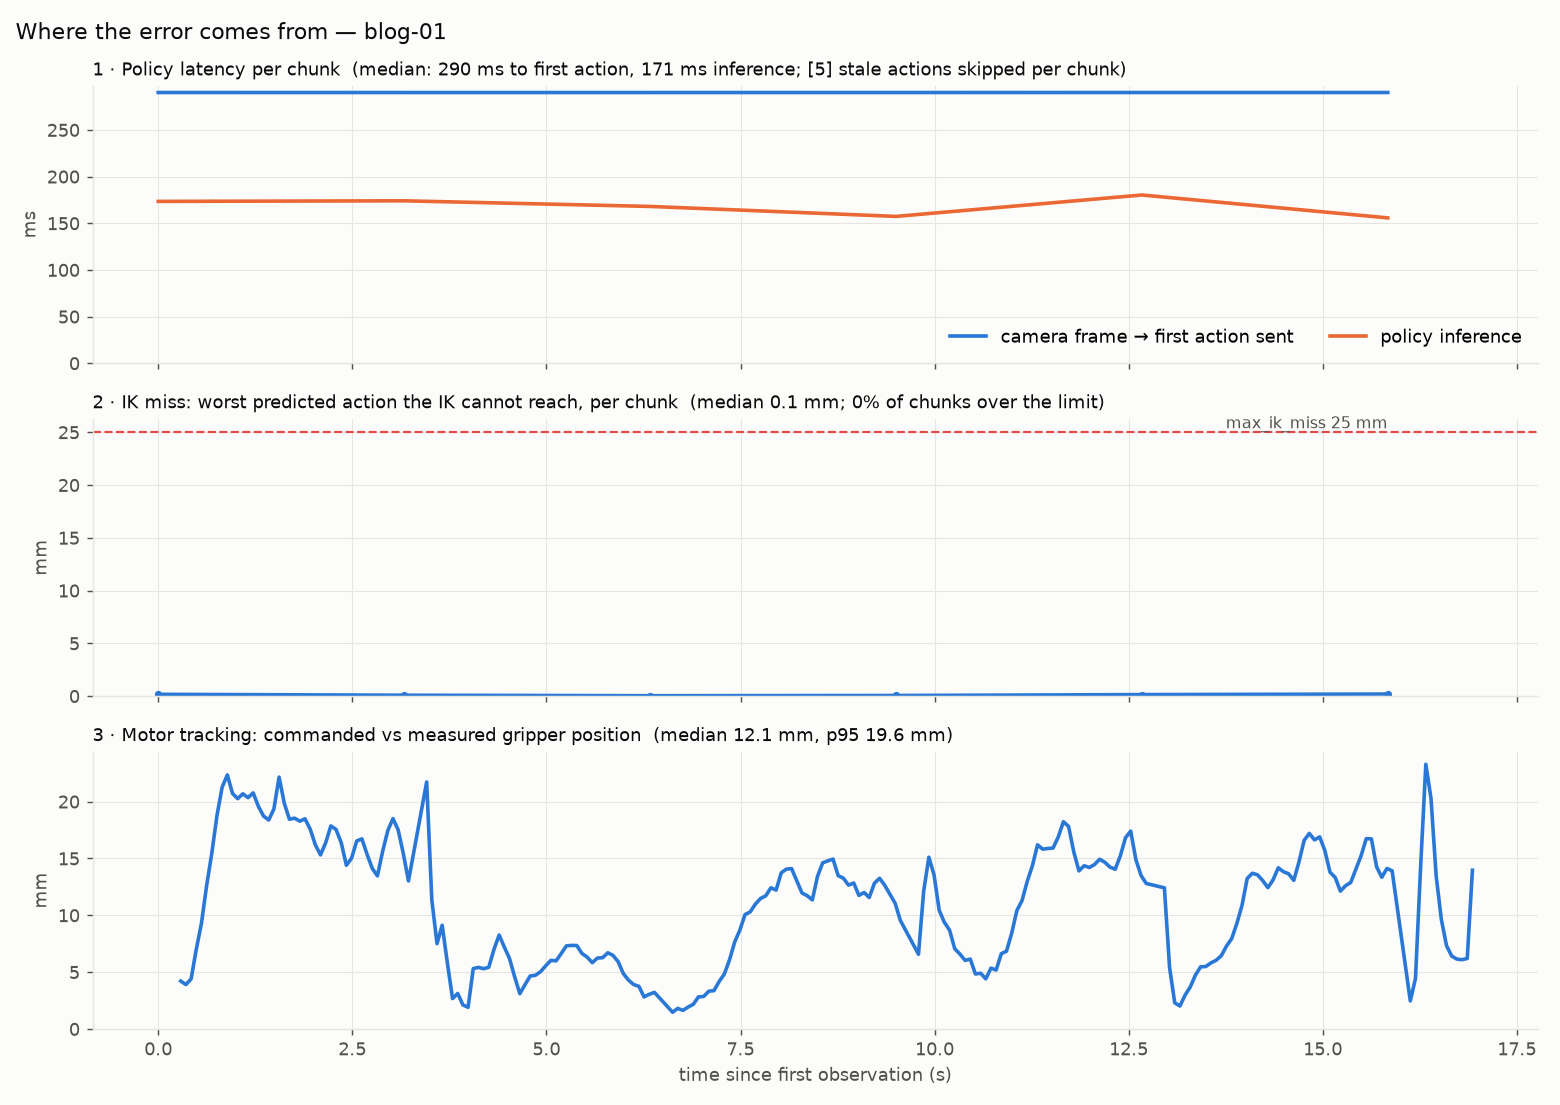
\includegraphics[width=\linewidth]{figures/rollout-pipeline.png}
\caption{One rollout: per-chunk latency, IK miss and motor tracking error.}
\label{fig:latency}
\end{figure}

\section{Limitations and next steps}
We have not measured a task success rate, and we have not yet shown that
IK-validated or re-placed data trains a better policy. That is the next
experiment: train on all, gated and re-placed data from the same sessions, and
compare success over repeated trials. The tracker-to-tool transform is assumed
from CAD and the camera-to-pose time offset is taken as zero rather than
measured. The workspace is kinematic only (no self- or table-collision), and on
one capture recorded with the assumed mount, the one-step QP follower started
from the default pose stalled at a joint limit after the placement fit while the
decoupled solver tracked 93\% of frames; joint-limit margin belongs in the
placement objective. Everything runs on one task with one arm.

\section{Conclusion}
With a stock arm, the arm's own model and IK can audit handheld data before any
training. Replaying demonstrations through the deployment IK exposes frames the
policy could never execute, a full-pose solver removes 38\% of those rejects and makes
accepted frames sub-millimetre, and a learned workspace turns reachability into a
microsecond query that can re-place demonstrations so every frame is executable.

\bibliographystyle{plainnat}
\bibliography{refs}
\end{document}
